\section{Case Study}
\label{sec:casestudy}

In modern distributed computing frameworks (e.g. MPI\cite{mpibook} and ZooKeeper\cite{JunqueiraZab2011}), \emph{leader election} plays an important role to organize multiple servers efficiently and consistently. This section shows how a classical leader election algorithm is modeled and reused to coordinate other components in \lang{}.

In \cite{HagitDistributed2004} the authors proposed a classical algorithm for a typical leader election scenario, as shown in Fig. \ref{fig:leaderelection}. Distributed processes are organized as an \emph{asynchronous unidirectional} ring where communication takes place only between adjacent processes and following certain direction (indicated by the arrows on edges in Fig. \ref{fig:leaderelection} (a)).

\begin{figure}
	\centering
	\resizebox{.7\textwidth}{!}{
        \tikzstyle{node}=[
    circle,
    draw
]

\begin{tikzpicture}[remember picture]
    \def \n {5}
    \def \radius {2cm}
    \def \margin {11} % margin in angles, depends on the radius

    \foreach \s in {1,...,\n}
    {
    \node[draw, circle] at ({360/\n * (\s - 1)}:\radius) {$P_\s$};
    \draw[<-, >=latex] ({360/\n * (\s - 1)+\margin}:\radius) 
        arc ({360/\n * (\s - 1)+\margin}:{360/\n * (\s)-\margin}:\radius);
    }

    \node[draw, rectangle, minimum width=4cm] at (6,0) {
        \begin{tabular}{c}
            \\
            Process ($P_i$) \\
             \\
            \begin{tikzpicture}[remember picture]
                \node [draw, rectangle, minimum width=3cm, minimum height=1cm] (connector) at (0,0) {\texttt{election\_module}};
            \end{tikzpicture} \\
            \\
            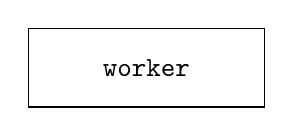
\begin{tikzpicture}[remember picture]
                \node [draw, rectangle, minimum width=3cm, minimum height=1cm] (component) at (0,0) {\texttt{worker}};
            \end{tikzpicture}
            \vspace{0.5em}
        \end{tabular}
        };
    
    \draw[->, >=latex] (3,0.3) -- (connector) node[midway, above, xshift=-0.35cm] {\texttt{left}} ;
    \draw[->, >=latex] (connector) -- (9,0.3) node[midway, above, xshift=0.3cm] {\texttt{right}};
    \draw[<->, >=latex] (component) -- (connector) ;

    \node[] at (0,-2.8) {(a)};
    \node[] at (6,-2.8) {(b)};
\end{tikzpicture}
    }
	\caption{(a) Topology of an Asynchronous Ring and (b) Structure of a Process}
	\label{fig:leaderelection}
\end{figure}

The algorithm has the following steps. At first, each process sends a voting message containing its own \emph{id} to its successor. When receives a voting message, the process will
\liyi{
	\emph{a)} forward the message to its successor if it contains a larger \emph{id} than the process itself, or
	\emph{b)} ignore the message if it contains a smaller \emph{id} than the process itself, or
	\emph{c)} take the process itself as a leader if it contains the same \emph{id} with itself, and send an acknowledgement message to this successor, which will be spread over around the ring. 
}

Here we formalize this algorithm through a more general approach. Leader election is encapsulated as the \texttt{election\_module}. A computing module \texttt{worker},  attached to the \texttt{election\_module}, is an implementation of the working process. 

Two types of messages, \texttt{msgVote} and \texttt{msgLocal}, are supported when formalizing this architecture. Voting messages \texttt{msgVote} are transferred between the processes. A voting message carries two fields, \emph{vtype} that declares the stage of leader election (either it is still voting or some process has already been acknowledged) and \emph{id} is an identifier of the current leader (if it exists). On the other hand, \texttt{msgLocal} is used when a process communicates with its corresponding worker.
\begin{example}[The Election Module] The following automaton shows how the election algorithm is implemented in \lang{}. Due to the space limit, we omit some transitions here. A full version can be found at \cite{medmodels}.
\begin{lstlisting}[basicstyle=\scriptsize\ttfamily]
automaton <id:int> election_module ( left : in msgVote, right : out msgVote,
	query : out msgLocal
) {
	variables {
		leaderStatus : enum { pending, acknowledged } init pending;
		buffer : (voteMsg | NULL) init {vtype: vote, id:id};
		leaderId : (int | NULL) init null;
	}
	transitions {
		(buffer != null)&&(buffer.vtype == vote)&&(buffer.id < id) -> {buffer := null;}
		(buffer != null)&&(buffer.vtype == vote)&&(buffer.id == id) -> {buffer.vtype := ack;}
		(buffer != null)&&(buffer.vtype == ack)&&(buffer.id < id) -> {
			// restart voting if the acknowledged leader has a smaller id
			buffer := { vtype: vote, id: id };
		}
		(buffer != null)&&(buffer.vtype == ack)&&(buffer.id >= id) -> {
			leaderStatus := acknowledged;
			leaderId := buffer.id;
			buffer := buffer.id == id ? null : buffer;
		}
	}
}
\end{lstlisting}
\end{example}


The following code fragment encodes a parallel program containing 3 \emph{worker}s and 3 \emph{election\_module}s to organize the \emph{worker}s.  In this example, we do not focus on the implementation details on \emph{worker}s, but hope that any component with a proper interface could be embedded into this system instead. 

\begin{lstlisting}[basicstyle=\scriptsize\ttfamily]
system <worker: interface (query:in msgLocal)> parallel_instance() {
	components {
		E1 : election_module<1>;
		E2 : election_module<2>;
		E3 : election_module<3>;
		C1, C2, C2 : worker;
	}	
	connections {
		Sync<msgVote>(E1.left, E2.right);
		Sync<msgVote>(E2.right, E3.left);
		Sync<msgVote>(E3.right,	E1.left);
		
		Sync<msgLocal>(C1,query,  E1.query);
		Sync<msgLocal>(C2,query,  E2.query);
		Sync<msgLocal>(C3,query,  E3.query);
	}
}
\end{lstlisting}

As we are modeling the leader election algorithm on a synchronous ring, only synchronous communication channels \emph{Sync}s are involved in this example. The implementation details of \texttt{Sync} can be found in  \cite{medmodels}.